\chapter{Java Management Extensions}
\label{ch:4}
\textit{Java Management Extensions} (JMX) é uma API que fornece uma maneira simples e padrão de gestão e monitoramento de recursos para a plataforma Java. Estes recursos podem ser aplicações, dispositivos, serviços ou a própria JVM (\textit{Java Virtual Machine}). São instrumentados por um ou mais \textit{Managed Beans}, ou simplemente Mbeans, resposáveis por adquir, manipular ou enviar informações sobre o recurso~\cite{lindfors2002jmx}.

Essa tecnologia foi desenvolvida através do JCP (\textit{Java Community Process}), em duas JSRs (\textit{Java Specification Request}) distintas. A JSR 3, \textit{Java Management Extensions Instrumentation and Agent Specification} e a JSR 160, \textit{Java Management Extensions Remote API}.

JCP é o processo de desenvolvimento padrão de novas especificações para a plataforma Java, as chamadas JRSs, que são documentos que descrevem as especificações e tecnologias propostas à plataforma.

A especificação de JMX define, além da arquitetura, padrões de projeto, API's e um conjunto de serviços de gerenciamento e monitoramento. Possibilitando o desenvolvimento de aplicações gerenciáveis local ou remotamente através do processo de instrumentação, onde atributos, configurações e capacidades da aplicação são expostos. Aumentando a robustez e extensibilidade da aplicação, uma vez que, é possível construir soluções de gerenciamento inteligentes, interoperáveis e independentes da infra-estrutura de gestão~\cite{jmx}.
\newpage

\section{Arquitetura}

A arquitetura JMX é definida em três níveis, ver Figura \ref{fig:arch_jmx}:

\begin{itemize}
 \item Nível de Instrumentação;
 \item Nível de Agente;
 \item Nível de Gerenciamento.
\end{itemize}

Como foi dito anteriormente, JMX foi definida segundo duas JSRs , JSR 3 e JSR 160. Os dois primeiros níveis da arquitetura (Intrumentação e Agente) foram definidos na JSR 3, enquanto o Nível de Gerenciamento foi definido na JSR 160. Isso mostra, de certa forma, o pontencial de extensibilidade da tecnologia.
\newline

\begin{figure}[htp]
\centering
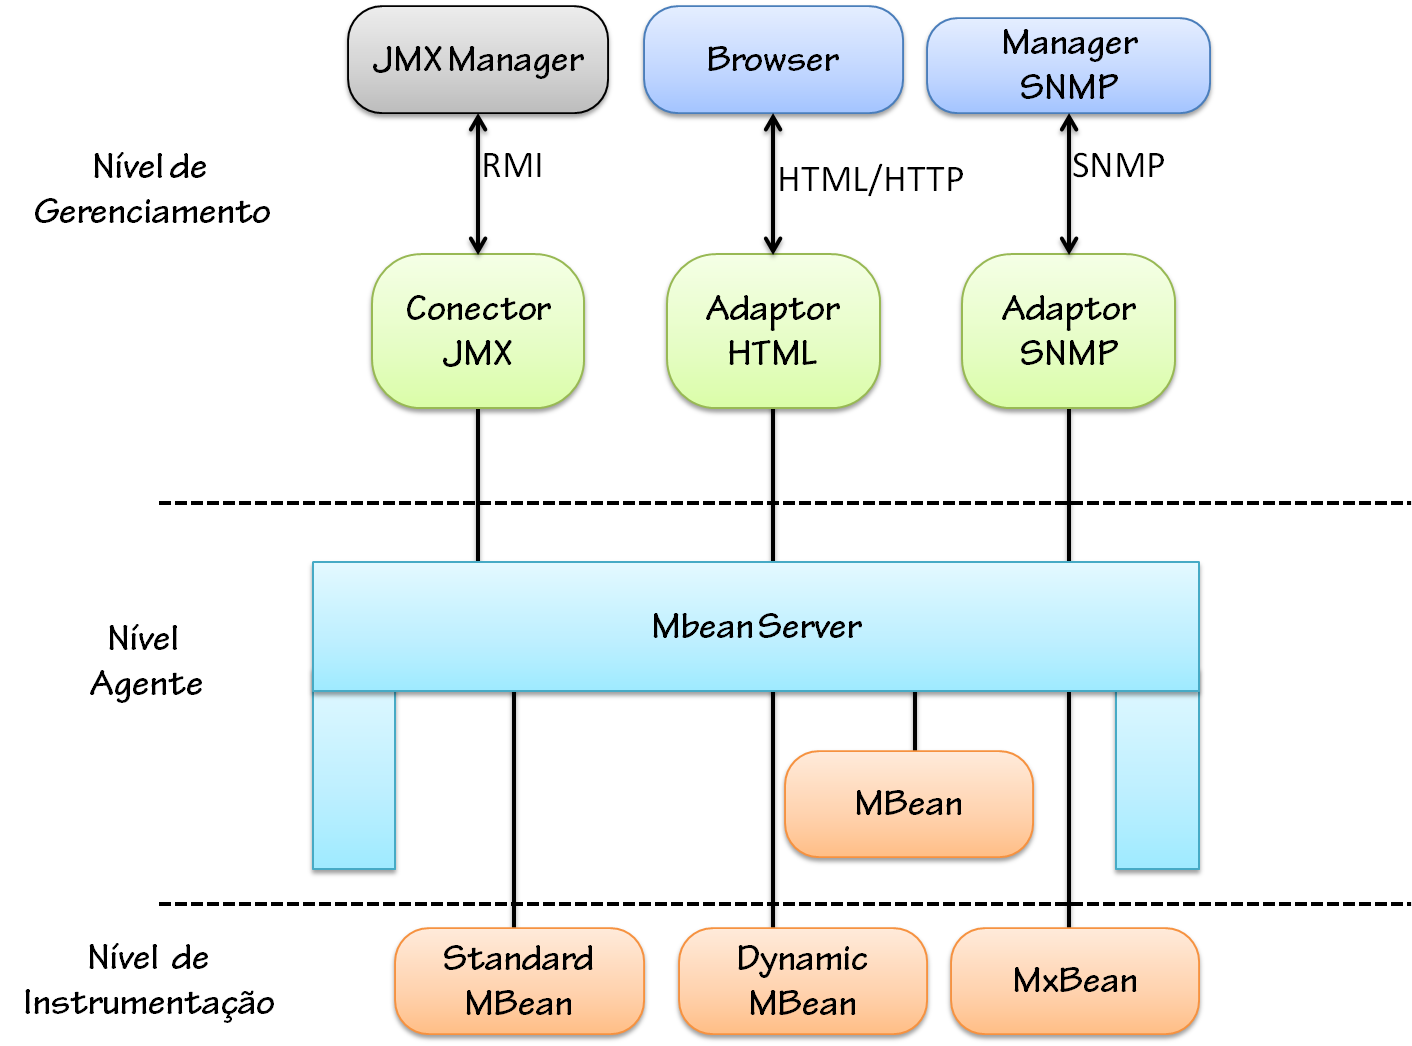
\includegraphics[width=12cm]{chapters/chapter4/arch_jmx.png}
\caption[Arquitetura JMX]{Arquitetura JMX.}
\label{fig:arch_jmx}
\end{figure}

\subsection{Nível de Intrumentação}
O nível de instrumentação é resposável por expor as funcionalidades e configurações das aplicações através da criação e registro de Mbeans. Estes Mbeans coletam e manipulam as informações dos recursos gerenciáveis, repassando-as aos agentes JMX do nível superior.

\subsection{Nível Agente}

\subsection{Nível de Gerenciamento}